\chapter{Analyse et Spécification des Besoins}
\label{ch:analyse_specifications}

\section{Introduction}
Ce chapitre formalise la traduction des contraintes juridiques issues de la loi algérienne 18-07, relative à la protection des personnes physiques dans le traitement des données à caractère personnel, et de la loi 25-11 sur la cybersécurité, en spécifications logicielles strictes. L'objectif est de définir l'architecture comportementale et fonctionnelle d'une plateforme de gouvernance des données selon le paradigme de \textit{Compliance by Design}, garantissant que les mécanismes de conformité et de sécurité s'imbriquent de manière native dans chaque couche du système.

\section{Identification des Acteurs du Système}
L'architecture de la plateforme repose sur une application rigoureuse du principe de séparation des tâches (\textit{Separation of Duties} - SoD) afin de limiter les risques de compromission interne. Le système isole les privilèges à travers quatre profils distincts, empêchant l'accumulation de droits critiques. 

\textbf{Le Responsable de Traitement (RT / Métier) :} Il s'agit de l'entité opérationnelle qui manipule la donnée personnelle au quotidien pour les besoins métiers. Son action sur le système se limite d'un point de vue transactionnel à la déclaration des nouveaux traitements, à la spécification des finalités et à l'exécution de l'activité cible. Ce profil ne possède aucune prérogative de validation réglementaire quant à la conformité de ses propres traitements.

\textbf{Le Délégué à la Protection des Données (DPO) :} Agissant en tant qu'auditeur interne et garant de la conformité légale, le DPO dispose d'un rôle exclusif de pilotage et de contrôle. Il valide ou rejette les traitements déclarés par le RT sur le plan juridique et orchestre la gestion des incidents. Ce profil de supervision ne possède structurellement aucune autorisation d'exécution sur le cycle de vie direct des données métier.

\textbf{Le Directeur de la Sécurité des Systèmes d'Information (DSSI) :} Le DSSI administre l'infrastructure matérielle et logicielle, déploie les politiques de sécurité globale et gère la matrice des habilitations par l'implémentation stricte d'un contrôle d'accès basé sur les rôles (RBAC). Toutefois, pour garantir une intégrité absolue de la confidentialité vis-à-vis des métiers, le système interdit, par construction, au DSSI toute lecture ou interception des données métier en clair.

\textbf{La Personne Concernée (Client / Employé) :} Il s'agit du propriétaire légitime de l'information exploitée. Cet acteur interagit avec le système de façon extrinsèque via un portail dédié, lui octroyant l'exercice transparent de ses droits légaux, sans intermédiation humaine superflue ni compromission des flux internes.

\section{Spécifications des Besoins Fonctionnels}
Le périmètre fonctionnel du système s'articule autour de l'industrialisation procédurale de la conformité légale au travers de fondations applicatives.

\textbf{Cartographie et Registre :} Le système centralise l'inventaire complet des traitements opérés au sein de l'organisme. Il permet l'identification systématique et la documentation dynamique de la nature des données collectées, de leurs finalités de traitement, des durées de conservation légales et de l'arborescence des destinataires internes ou externes.

\textbf{Guichet Unique des Droits (DSAR) :} La plateforme implémente un module de gestion automatisée des requêtes (\textit{Data Subject Access Request}). Elle autorise et simplifie l'encapsulation de concert des processus de demande d'accès, de rectification et de suppression. Cette automatisation requiert systématiquement la vérification mathématique de l'identité du demandeur au moyen d'une authentification forte multifacteur (MFA).

\textbf{Assistance Juridique Souveraine :} Afin d'éprouver la pertinence des décisions de conformité, la plateforme embarque localement un Grand Modèle de Langage (LLM), couplé à une architecture de génération augmentée par la recherche (RAG). Ce moteur d'inférence indexe les corpus législatifs afin d'évaluer de façon analytique les Études d’Impact sur la Vie Privée (AIPD) et guide le DPO face aux cas jurisprudentiels complexes. 

\textbf{Gestion des Violations :} En adéquation avec le cadre punitif de la Loi 18-07, le système déploie un workflow automatisé de réponse à incident de sécurité. Dès la détection formelle d'une compromission de données, l'application initie une cascade de procédures d'alerte à destination de l'Autorité Nationale de Protection des Données à Caractère Personnel (ANPDP), activant un déclencheur horodaté garantissant le respect de la notification légale sous un délai implacable de 120 heures.

\section{Spécifications des Besoins Non-Fonctionnels}
Les propriétés non-fonctionnelles du système traduisent les directives impérieuses de cybersécurité en garanties techniques infranchissables.

\textbf{Sécurité et Souveraineté :} L'architecture impose un hébergement strictement \textit{On-Premise}. Le déploiement s'articule au sein d'une infrastructure locale close. Aucune télémétrie, ni externalisation computationnelle, et surtout aucun transfert vers un fournisseur Cloud étranger n'est toléré, fixant formellement l'empreinte logicielle et juridique sous seule juridiction et souveraineté algériennes.

\textbf{Traçabilité Inaltérable :} Reposant sur une base de données optimisée pour l'ajout permanent (\textit{Write Once Read Many} - WORM), la plateforme fige les journaux d'audit de manière inaltérable. La moindre interaction ou transition d'état sur un jeu de données sensible, couvrant chaque étape de création, lecture, mise à jour ou destruction (opérations CRUD), est immédiatement tracée, horodatée de manière déterministe et associée à une signature cryptographique pour valider la chaîne de confiance de l'audit.

\textbf{Chiffrement au Repos et Cloisonnement :} Conformément à la loi 25-11, les données bénéficient d'une sécurité maximale conjuguant un chiffrement symétrique puissant, standardisé AES-256 pour bloquer l'extraction des données hébergées au repos, ainsi qu'un chiffrement asymétrique protégeant la solidité des clés et des transferts. Parallèlement, le stockage lui-même obéit à une ségrégation physique et un cloisonnement logique sans faille, prohibant l'escalade transactionnelle non autorisée entre les départements de l'organisme.

\section{Modélisation des Cas d'Utilisation}
Afin de projeter la gouvernance des interactions fonctionnelles étudiées, le diagramme des cas d'utilisation ci-dessous modélise le spectre opérationnel alloué à chaque acteur identifié. Ce diagramme cristallise formellement le paradigme conceptuel du \textit{Compliance by Design} : il démontre structurellement que l'exhaustivité des processus métiers est invariablement interceptée, supervisée et contrainte par le noyau inviolable de sécurité et d'audit du système, plaçant le respect législatif non plus comme une posture déclarative, mais bien comme l'unique condition d'exécution de la plateforme.
\begin{figure}[H]
    \centering
    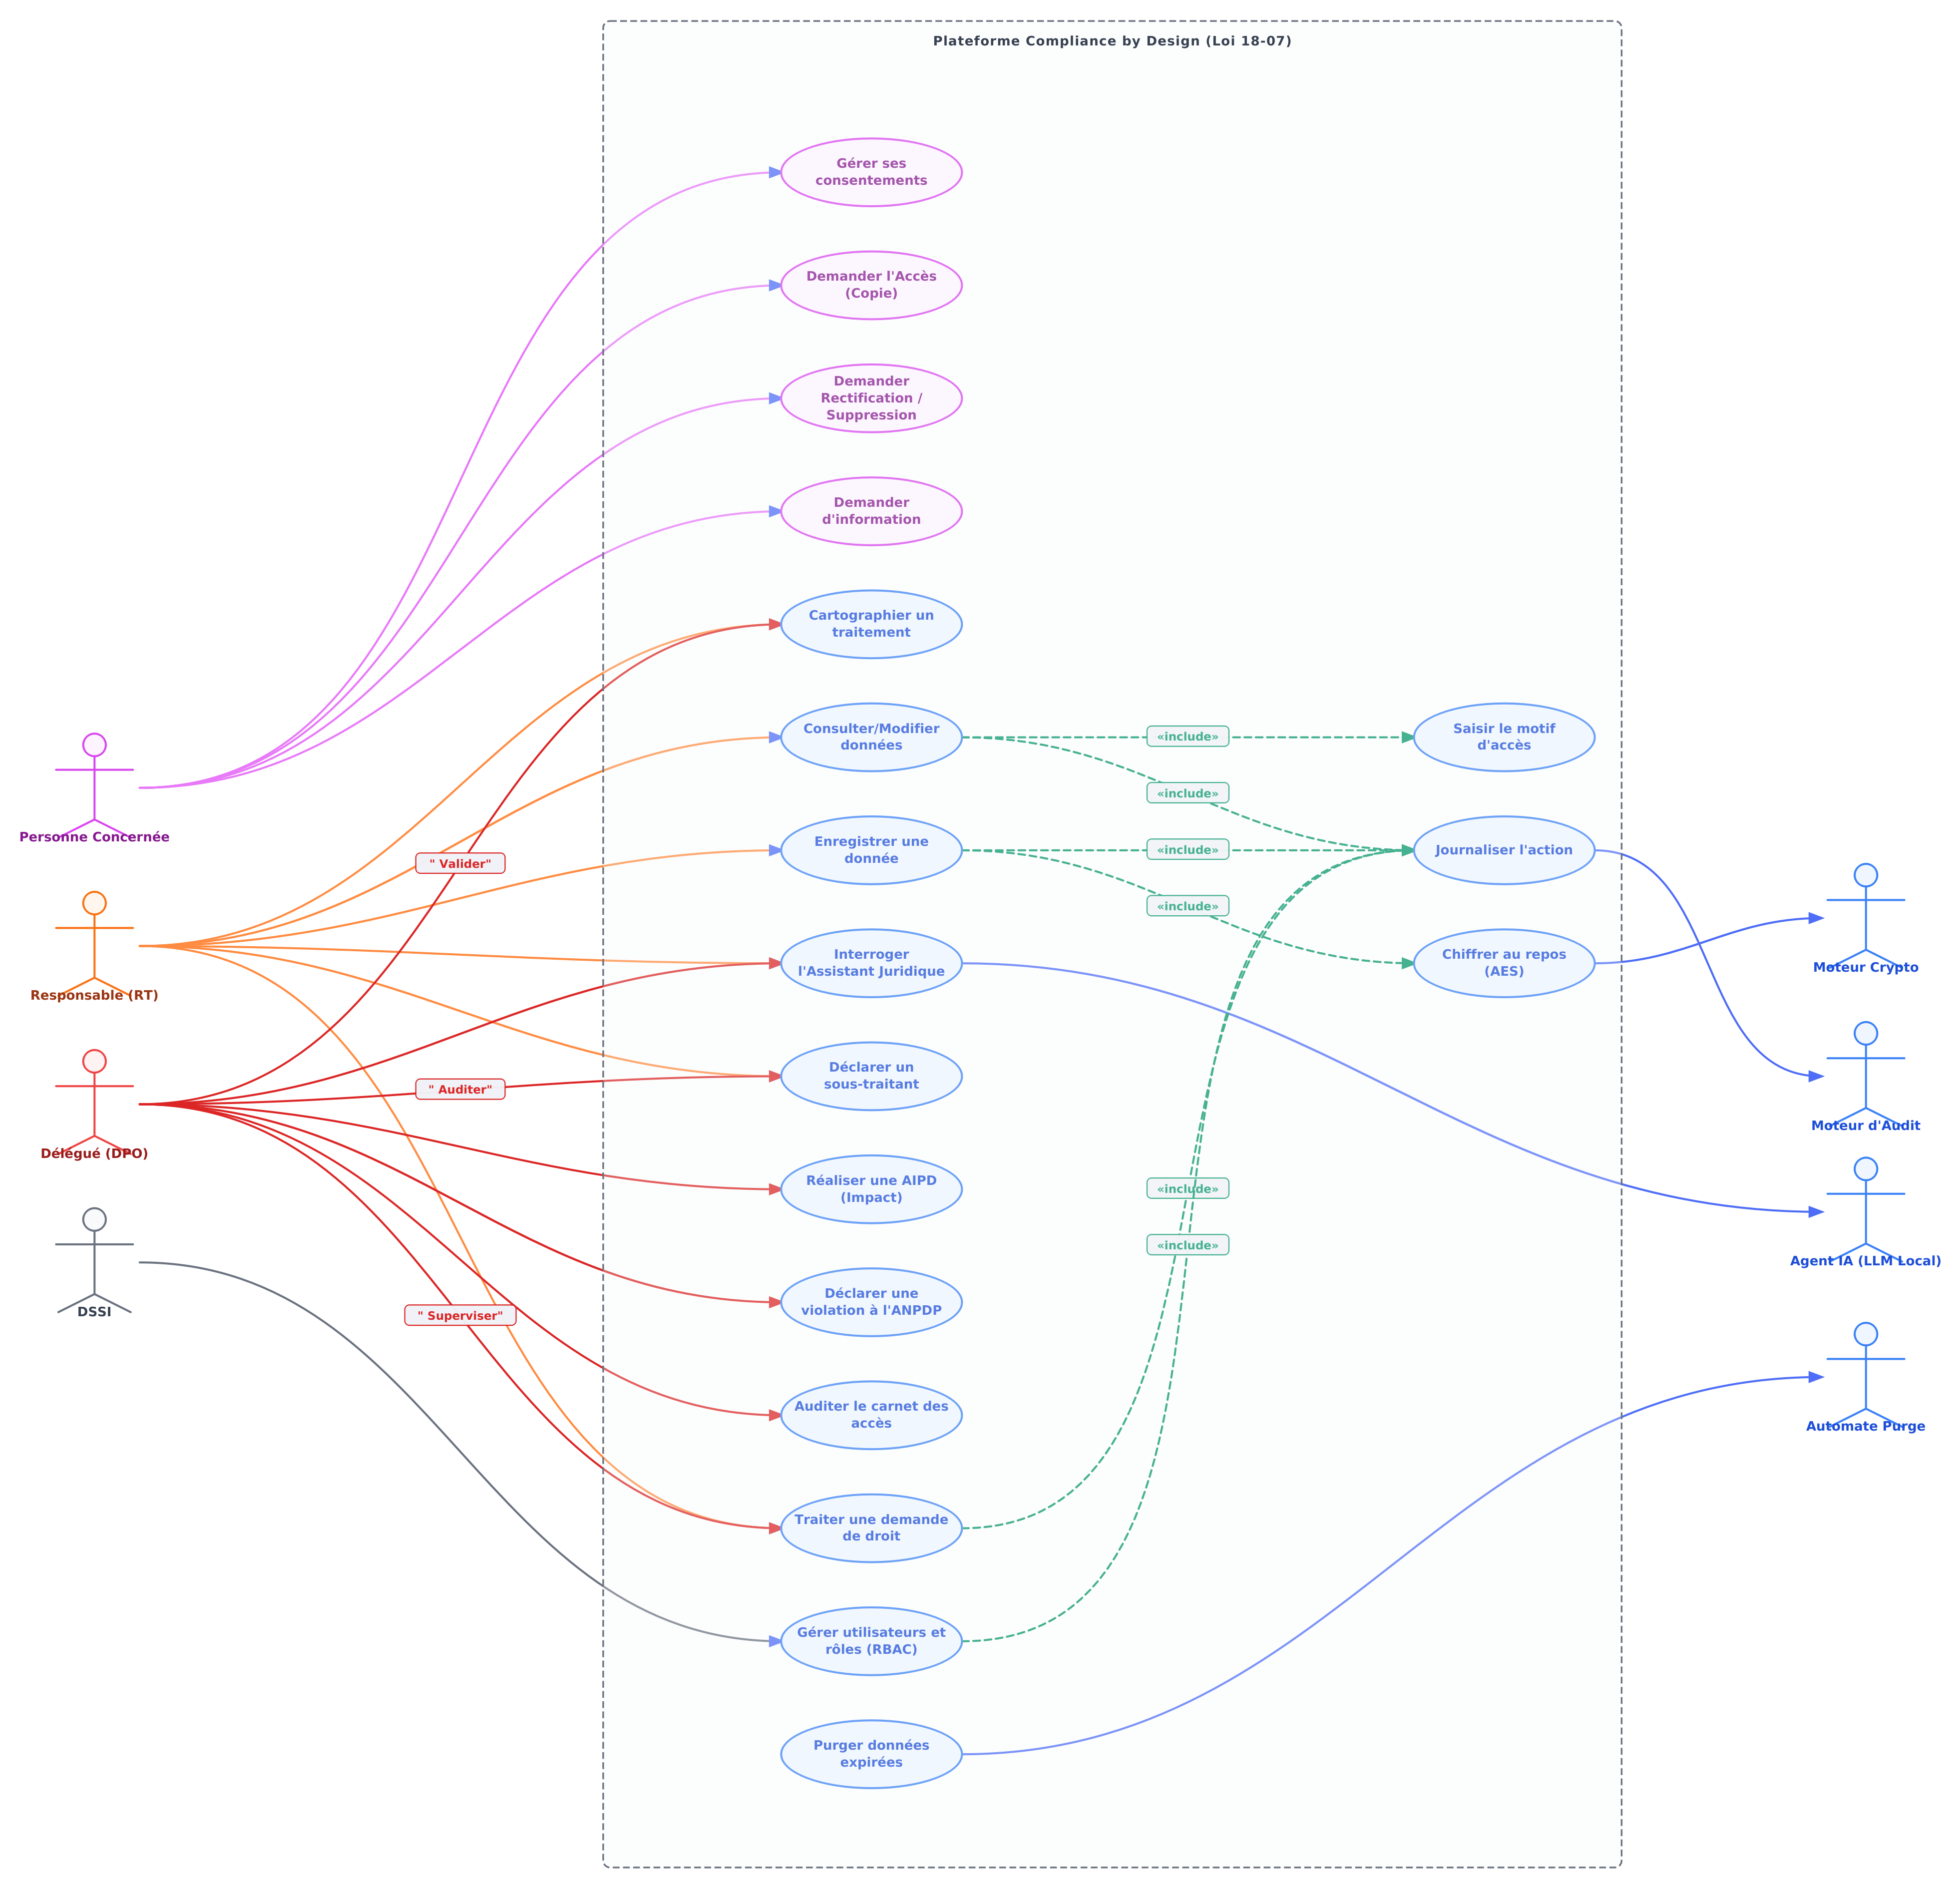
\includegraphics[width=\textwidth]{5-Chapters/Chapter2/DCU.png}
    \caption{Diagramme des Cas d'Utilisation de la Plateforme (Compliance by Design)}
    \label{fig:dcu_chapter2}
\end{figure}